\documentclass{article} % For LaTeX2e
\usepackage[legalpaper, margin=0.5in]{geometry}
\usepackage{amsmath}
\usepackage{amsfonts,dsfont}
\usepackage{amssymb}
\usepackage[ruled,vlined]{algorithm2e}

\usepackage{graphicx}
\usepackage{caption}
\usepackage{subcaption}
\usepackage{xcolor}

\begin{document}

\section{Simple GAN vs. Unsupervised Conditional GAN}
\begin{figure}[h]
	\centering
	\captionsetup{labelformat=empty}
	\begin{subfigure}[b]{0.3\textwidth}
		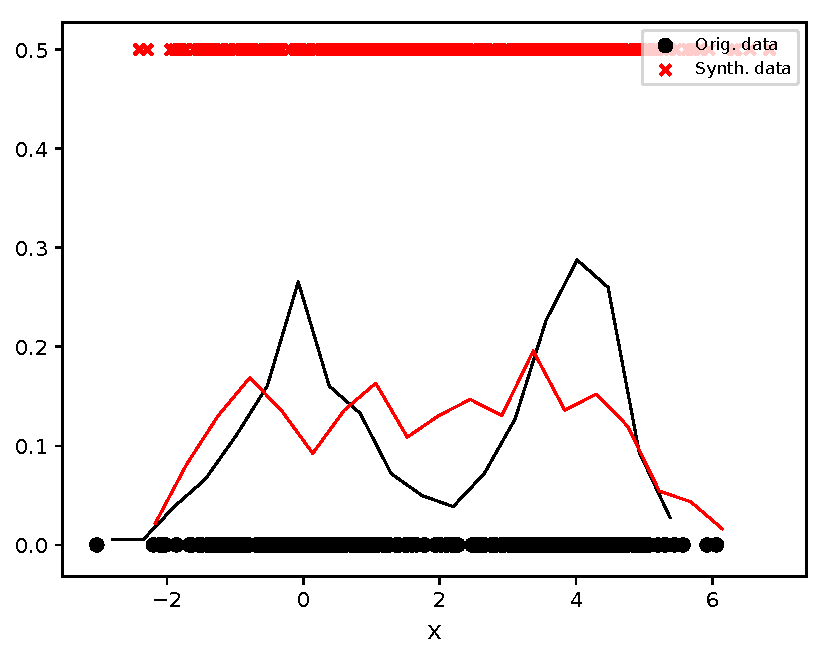
\includegraphics[width=\textwidth]{2_gan_ls9_1000_1000.pdf}
		\caption{Simple GAN (2 modes)}
		\label{fig:gan_2}
	\end{subfigure}
	\begin{subfigure}[b]{0.3\textwidth}
		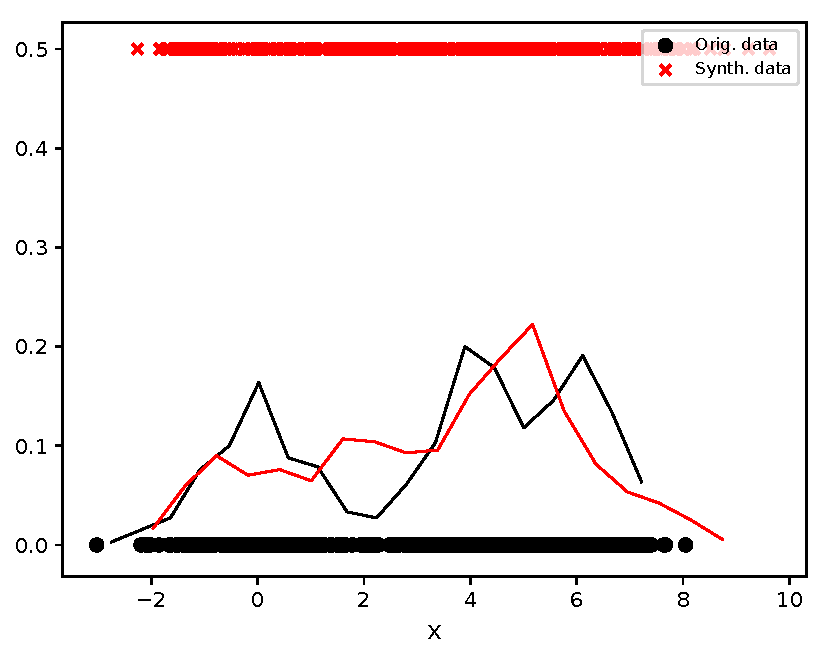
\includegraphics[width=\textwidth]{3_gan_ls9_1000_1000.pdf}
		\caption{Simple GAN (3 modes)}
		\label{fig:gan_3}
	\end{subfigure}
	\begin{subfigure}[b]{0.3\textwidth}
		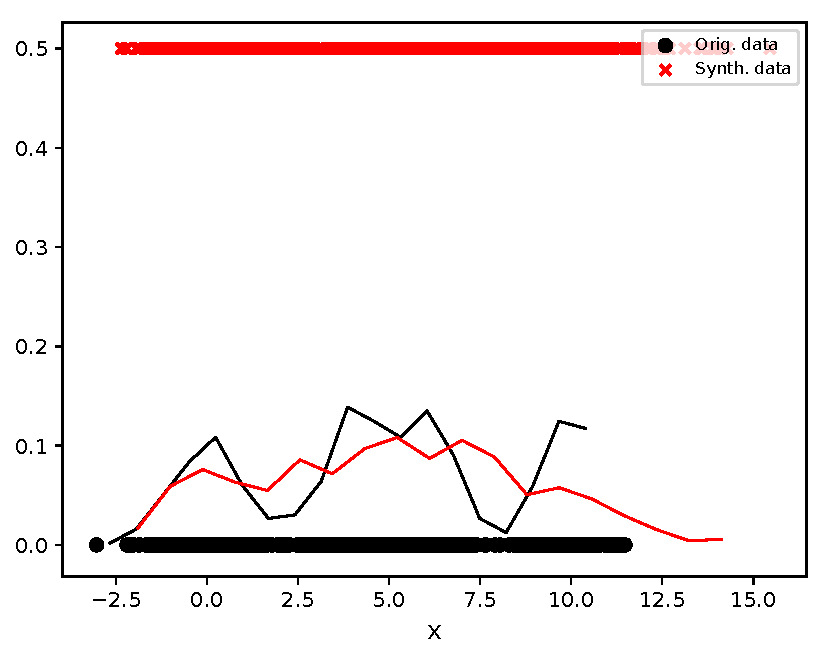
\includegraphics[width=\textwidth]{4_gan_ls9_1000_1000.pdf}
		\caption{Simple GAN (4 modes)}
		\label{fig:gan_4}
	\end{subfigure} \\
	\begin{subfigure}[b]{0.3\textwidth}
		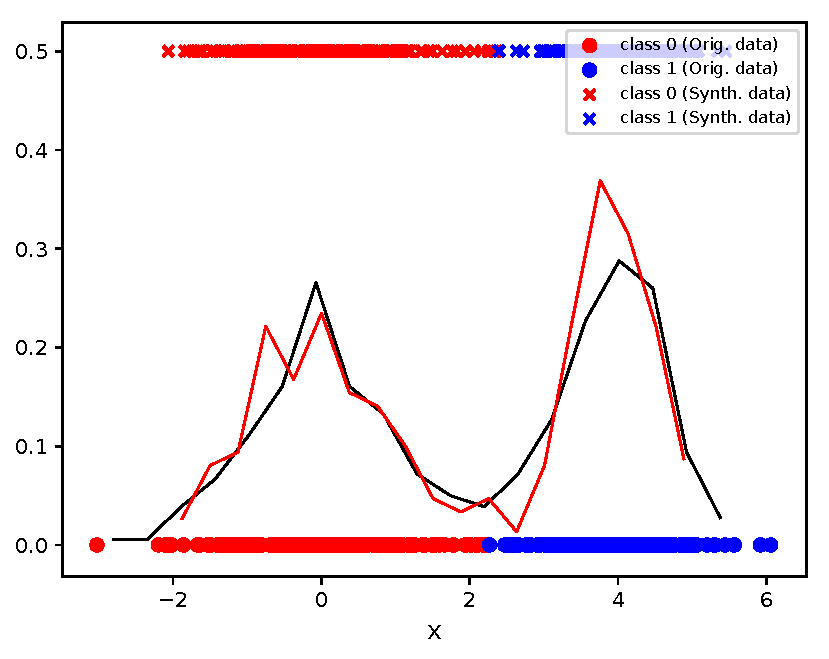
\includegraphics[width=\textwidth]{2_cond_gan_k2_ls9_1000_1000.pdf}
		\caption{Conditional GAN (2 modes)}
		\label{fig:cgan_2}
	\end{subfigure}
	\begin{subfigure}[b]{0.3\textwidth}
		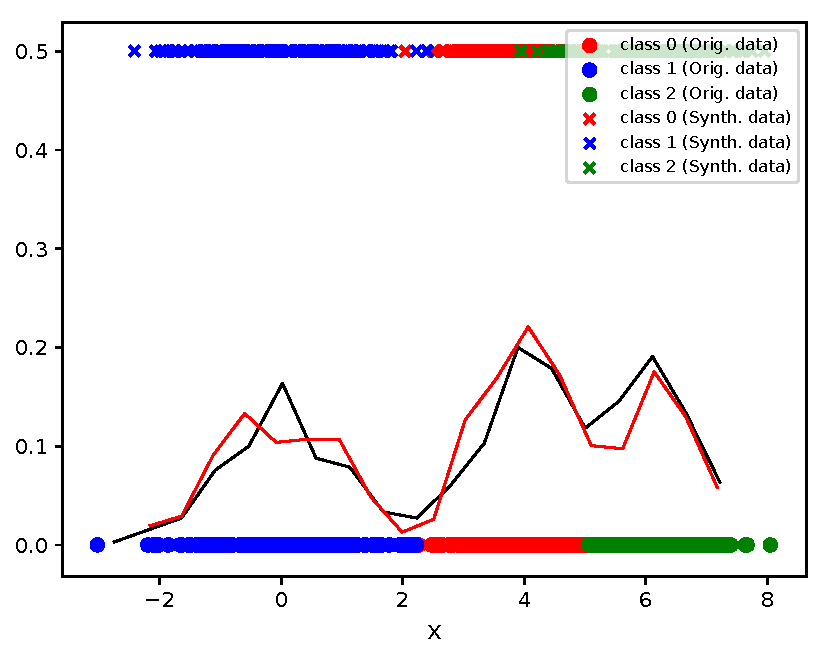
\includegraphics[width=\textwidth]{3_cond_gan_k3_ls9_1000_1000.pdf}
		\caption{Conditional GAN (3 modes)}
		\label{fig:cgan_3}
	\end{subfigure}
	\begin{subfigure}[b]{0.3\textwidth}
		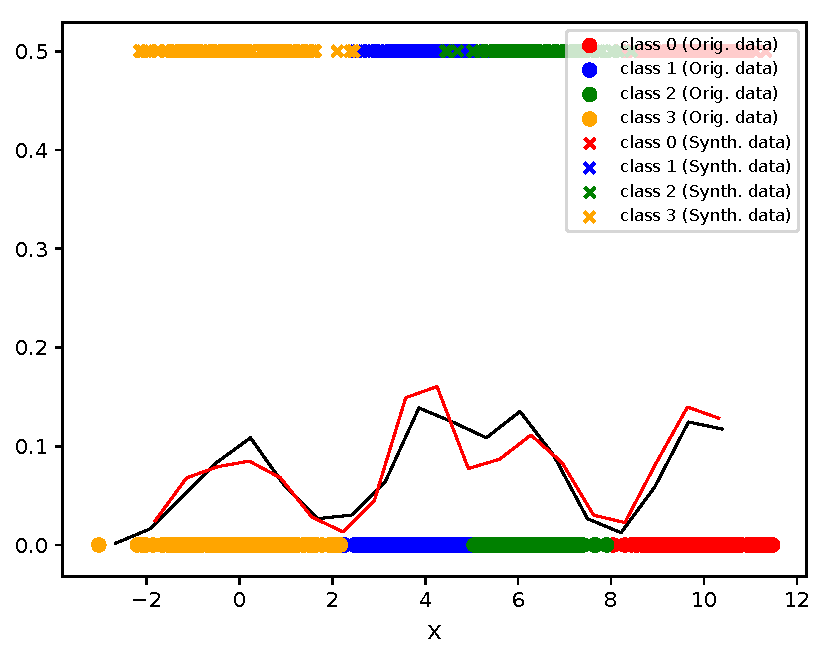
\includegraphics[width=\textwidth]{4_cond_gan_k4_ls9_1000_1000.pdf}
		\caption{Conditional GAN (4 modes)}
		\label{fig:cgan_4}
	\end{subfigure} \\[-1ex]
	\caption{Comparison between simple GAN and {\bf unsupervised} Conditional GAN (cGAN) for $1D$ data with multiple modes. The samples at $y=0$ are the real samples on which the GAN was trained. The samples at $y=0.5$ are synthetic samples generated by the GANs after training for $1000$ epochs. The {\em black} lines show the histogram of the original data. The \textit{\textcolor{red}{red}} lines show the histogram of the synthetic samples generated by the GAN. For the unsupervised cGAN, we first perform {\em unsupervised} clustering with Gaussian Mixture Models. The number of components were selected with {\em BIC}. The cluster labels are then assigned as the class labels. For the 1D data shown here, cluster information seems to help.}
	\label{fig:1d_gan}
\end{figure}

\section{AnoGAN}
\begin{figure}[h]
	\centering
	\captionsetup{labelformat=empty}
	\begin{subfigure}[b]{0.45\textwidth}
		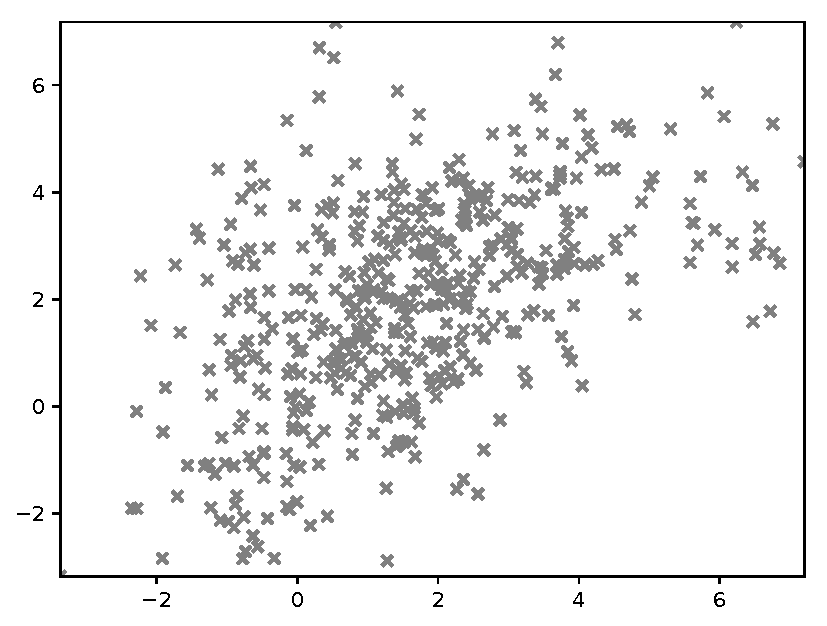
\includegraphics[width=\textwidth]{toy2_ano_gan_ls9_2000.pdf}
		\caption{Toy data samples}
		\label{fig:toy}
	\end{subfigure}
	\begin{subfigure}[b]{0.45\textwidth}
		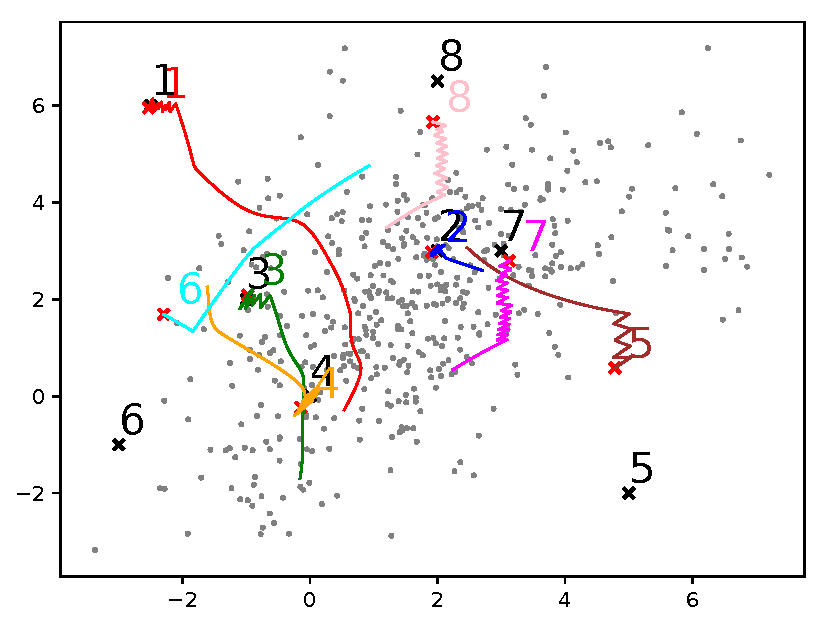
\includegraphics[width=\textwidth]{toy2_ano_gan_ls9_2000_test_ano_50.pdf}
		\caption{{\em AnoGAN} with simple GAN}
		\label{fig:gan_ano}
	\end{subfigure} \\
	\begin{subfigure}[b]{0.45\textwidth}
		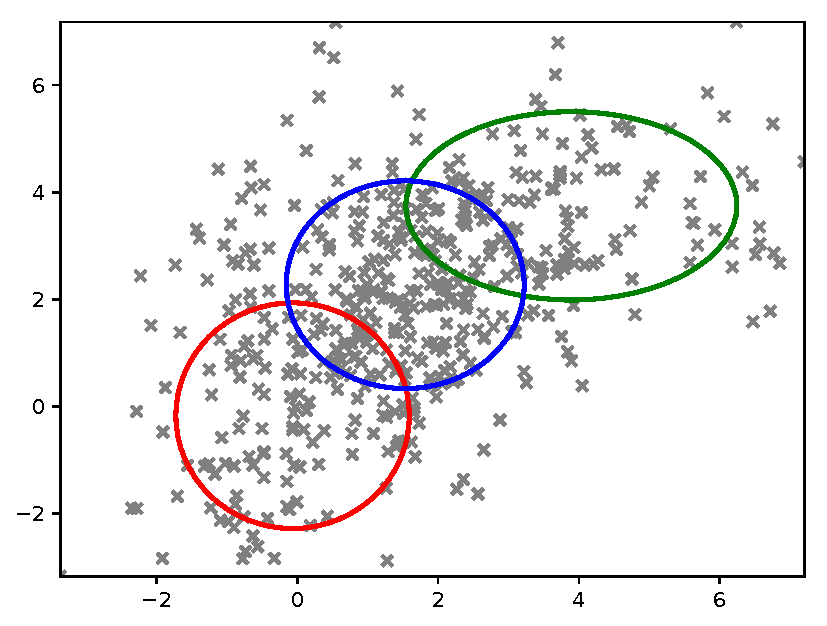
\includegraphics[width=\textwidth]{toy2_cond_ano_gan_k3_ls9_2000.pdf}
		\caption{Clusters for cGAN}
		\label{fig:cgan_k}
	\end{subfigure}
	\begin{subfigure}[b]{0.45\textwidth}
		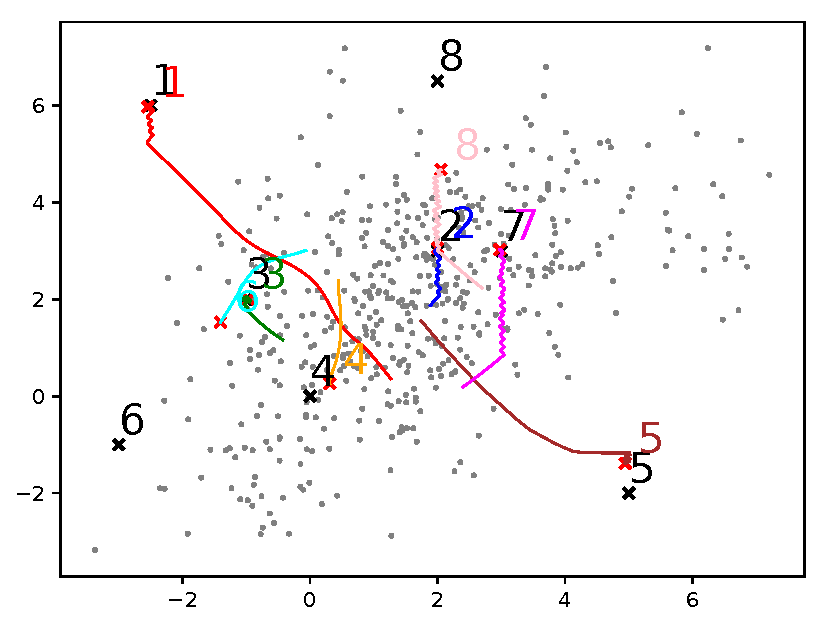
\includegraphics[width=\textwidth]{toy2_cond_ano_gan_k3_ls9_2000_test_ano_50.pdf}
		\caption{{\em AnoGAN} with cGAN}
		\label{fig:cgan_ano}
	\end{subfigure} \\[-1ex]
	\caption{Illustration of {\bf AnoGAN}. {\bf (a)} shows the $2D$ {\em Toy} data. All GANs were trained for $2000$ epochs. {\bf (b)} shows the AnoGAN results with a simple GAN. {\bf (c)} shows the unsupervised clustering of the {\em Toy} dataset. The number of components in the Gaussian Mixture Model was found to be $3$ using the $BIC$ model selection criteria. {\bf (d)} shows the AnoGAN results with a cGAN where the labels were assigned according to the clusters shown in {\bf (c)}. In {\bf (b)} and {\bf (d)} the points marked in {\em black} are test data points which were not available during training. Each test point has a corresponding colored point (marked with a \textit{\textcolor{red}{red `$\times$'}}) that represents its synthetic image reconstructed by AnoGAN. In simplistic terms, the distance between a test point and its reconstructed image can be considered a measure of anomalousness. {\bf (b)} and {\bf (d)} show that the points in the dense regions (e.g., $2, 3, 4, 7$) generally have low reconstruction loss. However, points in low-density regions (e.g., $1, 5, 6, 8$) give mixed results: while the reconstruction loss for $1$ is low, it is high for $5, 6, 8$. {\bf (b)} and {\bf (d)} also show the trace of reconstruction for each data point. AnoGAN computes the reconstructed image iteratively. For example, with test point $5$, the initial random latent representation $z_0$ corresponds to a point in the middle. After optimizing the AnoGAN loss, a new latent representation $z_1$ is found which corresponds to a point slightly closer to $5$. Then, using $z_1$ and optimizing, the next latent representation $z_2$ is found. Over the several iterations, the reconstructed image for $5$ moved along the \textcolor{brown}{brown} line until it finally reached the point marked with \textcolor{red}{$\times$}. The traces are useful for debug: we can see that all reconstructed points move closer to the target test points irrespective of where they start. It is hard to see whether a cGAN performs better than a simple GAN in this case. Moreover, the AnoGAN loss should be averaged over multiple runs for each test point because there is stochasticity in the initial latent representation.}
	\label{fig:ano_gan}
\end{figure}


\end{document}
